\documentclass[oneside,a4paper,12pt]{article}
% ---------------- Para Modificar ---------------- 
\newcommand{\principal}{Volumes}
\newcommand{\conteudo}{}
\newcommand{\turmas}{3~EMSI~A e do 3~EMSI~B}

\date{abril de 2021}

\newcommand{\citacao}{Que nada nos defina. Que nada nos sujeite. Que a liberdade seja a nossa própria substância.}
\newcommand{\autorcitacao}{Simone de Beauvoir}
% ------------------------------------------------

%-------------------------------------------------
\usepackage[english,brazilian]{babel}
\usepackage[alf]{abntex2cite}
\usepackage[utf8]{inputenc}
\usepackage[T1]{fontenc}
\usepackage[top=15mm, bottom=15mm, left=10mm, right=10mm]{geometry}
\usepackage{framed,booktabs,color,hyperref,graphicx}
\usepackage{amsfonts,amsthm,cancel}
\usepackage{subfigure,enumerate,float}
  
\definecolor{shadecolor}{rgb}{0.8,0.8,0.8}
\pagenumbering{arabic}

% Colunas
\usepackage{multicol}
\columnsep=10mm %Espaçamento entre colunas.
\setlength{\columnseprule}{1pt}

% Cabeçalho
\usepackage{fancyhdr}
\pagestyle{fancy}
\lhead{\textbf{\principal}}
\rhead{}
\renewcommand{\headrulewidth}{1pt} % espessura da linha do cabeçalho
\renewcommand{\footrulewidth}{1pt} % espessura da linha do rodapé

% Parágrafo
\setlength{\parindent}{1.25cm}

\newtheorem{problema}{Problema}
\newtheorem{exercicio}{exercicio}
\newtheorem{exemplo}{Exemplo}
\newtheorem{questao}{Questão}

\usepackage[skip=10pt]{caption}
\captionsetup{font={stretch=0.4,small}}

\newcommand{\FRASE}{\textit{``\citacao ''}\\(\textbf{\autorcitacao})}

\title{\LINHAHORIZONTAL \\\textbf{\\ \principal}\footnote{Resumo para os estudos das aulas não presenciais no período de quarentena para as turmas do \turmas .}\\\LINHAHORIZONTAL}

\newcommand{\LINHAHORIZONTAL}{\center \rule{16cm}{1.25pt}}
\newcommand{\sol}{\textbf{Solução}}

\newcommand{\m}[1]{\(\displaystyle {#1}\)}
\newcommand{\M}[1]{\[{#1}\]}

\author{\textbf{Professor Leandro Vieira}\\EREM Regina Pacis\\Palmeirina-PE}
\newcommand{\frase}{\begin{verse} \flushright{\FRASE} \end{verse}}


\begin{document}
\begin{enumerate}

\item O gráfico a seguir traz informações sobre o número de escolas por região que fazem parte da rede do PRONATEC.

\begin{figure}[!hbt]
\begin{multicols}{2}
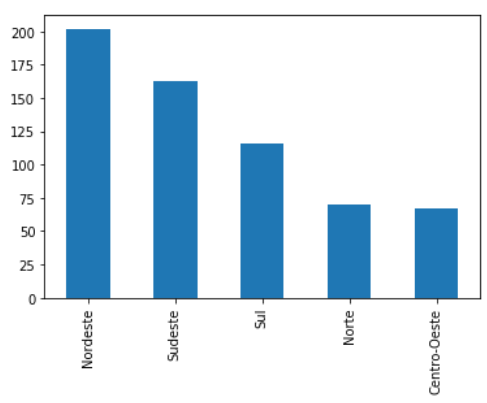
\includegraphics[width=8cm]{g01}

\columnbreak
\begin{enumerate}
\item Qual região apresenta o maior número de escolas na rede do PRONATEC?
\item Estime o número de escolas da região sudeste:
\item A região Norte tem o mesmo número de escoras da região Centro-Oeste? Justifique sua resposta:
\end{enumerate}
\end{multicols}
\end{figure}

\item No Gráfico a seguir são apresentados dados sobre o número de escolas por estado na rede do PRONATEC.

\begin{figure}[!hbt]
\begin{multicols}{2}
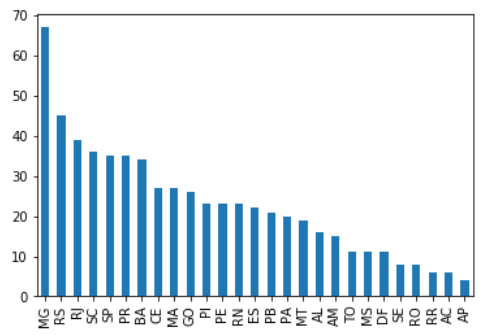
\includegraphics[width=8cm]{g02}

\columnbreak
\begin{enumerate}
\item Qual estado tem o menor número de escolas;
\item Qual a estimativa para o número de escolas do estado de Pernambuco.
\item Qual dos estados apresente o maior número de escolas:
\end{enumerate}
\end{multicols}
\end{figure}

\item O Gráfica a seguir apresenta informações sobre o número de partos cesarianos realizados em hospitais do Distrito Federal em janeiro de 2017

\begin{figure}[!hbt]
\begin{multicols}{2}
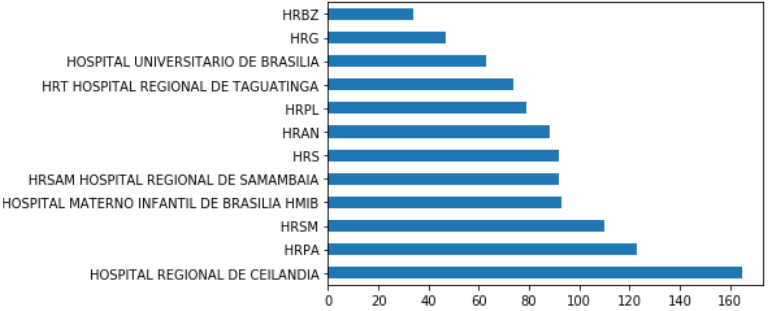
\includegraphics[width=10cm]{g03}

\columnbreak
\begin{enumerate}
\item Qual a estimativa de aprtos cesarianos para no hospital com menor incidência desse tipo de parto:
\item Qual o hospital apresentou um maior números de partos cesarianos? 
\end{enumerate}
\end{multicols}
\end{figure}

\newpage
\item A seguir é apresentado um gráfico com números sobre a quantidade de cursos integrantes do PROUNI por estado em 2018.

\begin{figure}[!hbt]
\begin{multicols}{2}
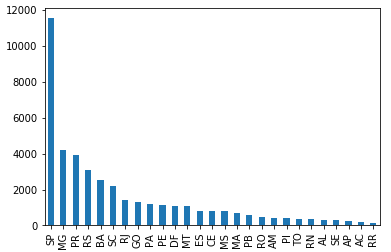
\includegraphics[width=10cm]{g04}

\columnbreak
\begin{enumerate}
\item Qual a estimativa da quantidade de cursos para o estado de Pernanbuco
\item Qual o estado com maior número de cursos, e o estado com o menor número de cursos.
\end{enumerate}
\end{multicols}
\end{figure}

\item Myanmar é um país do sul da Ásia continental que faz divisa, dentre outros países, com a China e  a Índia. Nos gráficos a seguir são apresentadas algumas informações sobre características da população 

\begin{figure}[!hbt]
\begin{multicols}{2}
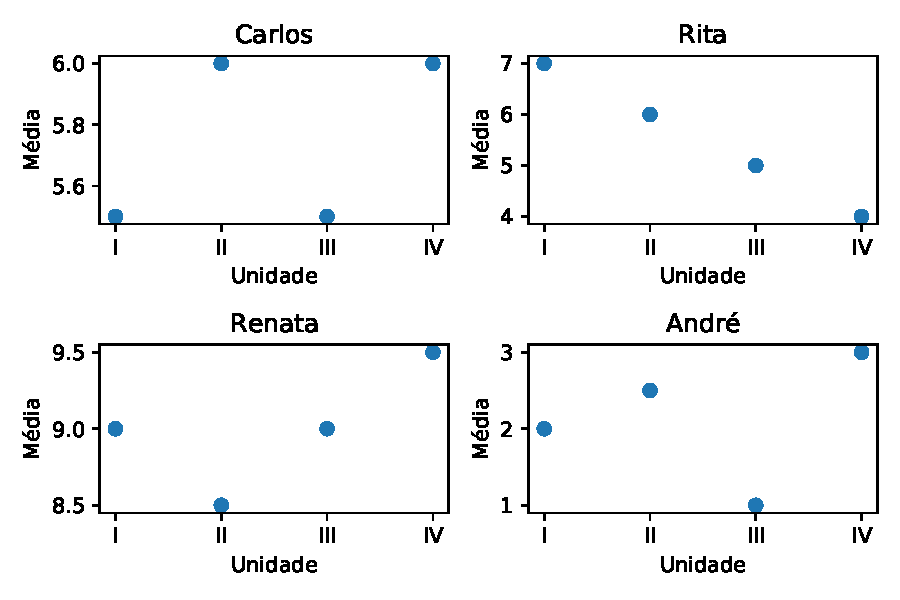
\includegraphics[width=4.5cm]{01}
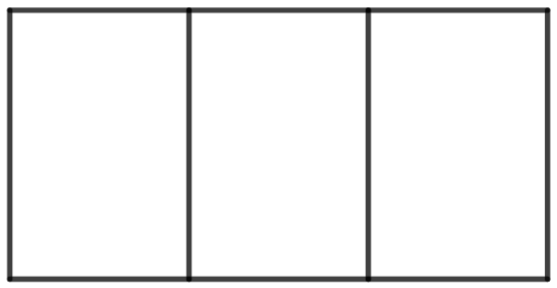
\includegraphics[width=4.5cm]{02}

De acordo com dados de 2014 sua população seria de aproximada 51.500.000. Com base nas informações apresentadas, resolva aos seguinte itens:
\begin{enumerate}
\item 

\item 
\end{enumerate}

\end{multicols}
\end{figure}

\newpage
\item O gráfico a seguir apresenta dados sobre faturamento de uma pequena lanchonete em cinco meses do ano de 2020.

\begin{figure}[!hbt]
\begin{multicols}{2}
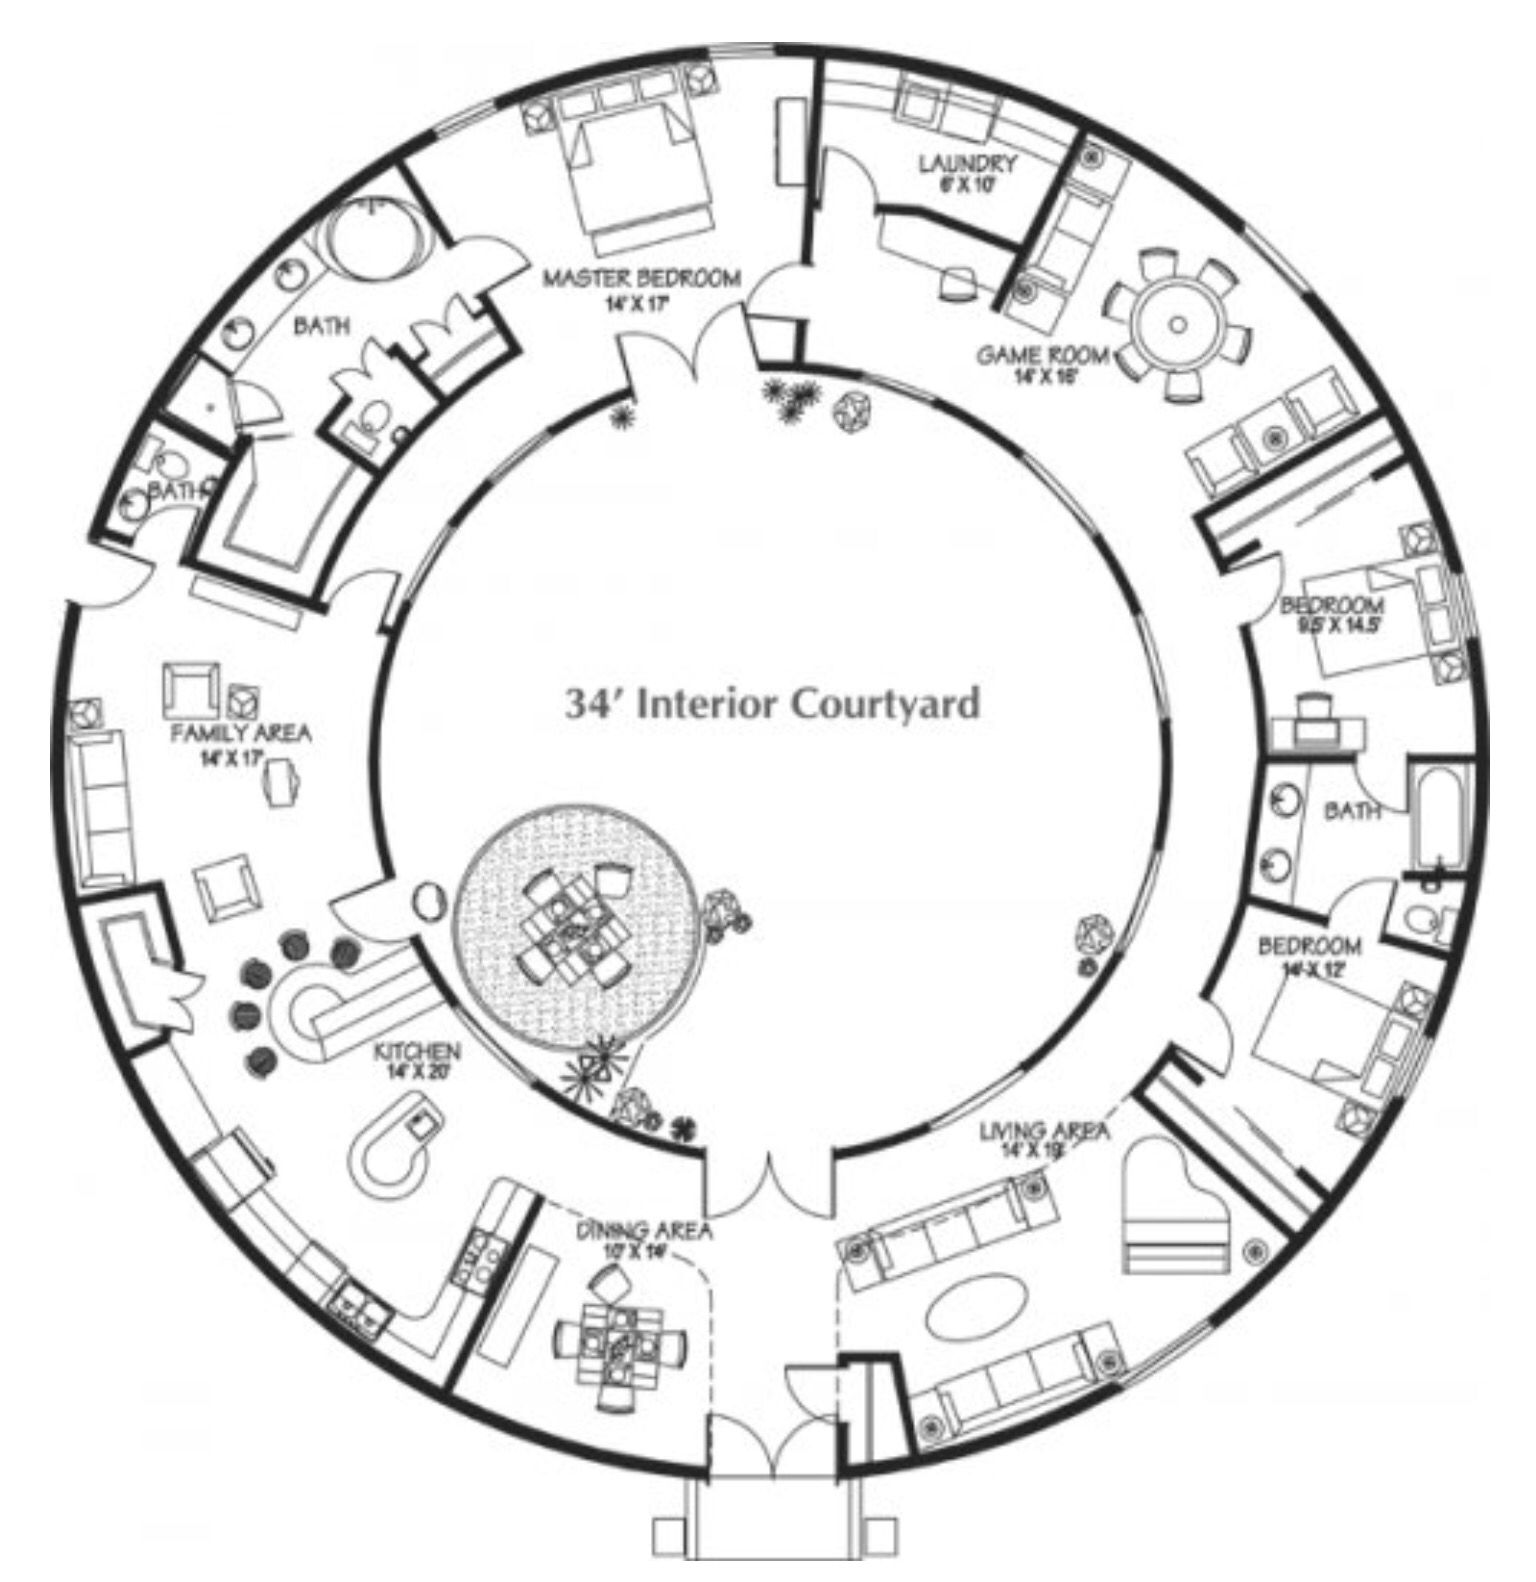
\includegraphics[width=10cm]{04}

\columnbreak
A coluna é o investimento em material e estrutura feito pelo dono da lanchonete, o gráfico em preto com linha contínua é o gráfico de lucro para os meses em questão, já o gráfico tracejado representa o faturamento na lanchonete no período observado:

Com base nas informações apresentadas na no gráfico resolva aos seguintes itens:
\begin{enumerate}
\item Em qual dos meses o lucro foi o maior? Qual o valor desse lucro? 
\item Em qual mês o faturamento foi o menor? Qual o valor do faturamento?
\item Existem meses que o faturamento foi o mesmo? Se sim, quais?
\item Existem meses que o lucro foi o mesmo? Se sim, quais?
\end{enumerate}

\end{multicols}
\end{figure}


\end{enumerate}
\end{document}